\documentclass[11pt,a4paper]{article}

\usepackage[margin=25mm]{geometry}
\usepackage{amsmath,amssymb}
\usepackage{graphicx}
\usepackage{booktabs}
\usepackage{hyperref}
\usepackage{enumitem}
\usepackage{xcolor}
\usepackage{tikz}
\usetikzlibrary{arrows.meta,positioning,shapes.geometric,fit}

% Monospace font: try to use Source Code Pro if available (pdflatex compatible)
% Note: pdflatex doesn't support fontspec, so we use a fallback approach
\IfFileExists{SourceCodePro-Regular.otf}{%
  \usepackage[default]{sourcecodepro}%
}{%
  \IfFileExists{inconsolata.sty}{%
    \usepackage{inconsolata}%
  }{%
    % Fallback to default monospace
  }%
}
% Make \texttt use monospace font consistently
\IfFileExists{SourceCodePro-Regular.otf}{%
  \newfontfamily\monofont{SourceCodePro-Regular.otf}[
    Path=./,
    BoldFont=SourceCodePro-Bold.otf,
    ItalicFont=SourceCodePro-Italic.otf
  ]
}{%
  \IfFileExists{inconsolata.sty}{%
    \usepackage[default]{inconsolata}%
    \let\monofont\ttfamily
  }{%
    \let\monofont\ttfamily
  }%
}
% Custom commands for DOI and paths (stylish monospace)
\newcommand{\doi}[1]{\href{https://doi.org/#1}{\monofont #1}}
% \localpath: handle underscores properly (escape them for LaTeX)
\newcommand{\localpath}[1]{\monofont \detokenize{#1}}
\let\oldtexttt\texttt
\renewcommand{\texttt}[1]{{\ttfamily #1}}

% --- Optional: embed example figures from the current "best run" ---
% Generated by: python3 docs/auto_pick_best_run.py
\IfFileExists{best_run_id.tex}{% Auto-generated by docs/auto_pick_best_run.py
\def\BestRunId{\detokenize{m1_check_np100_ns15}}
}{\def\BestRunId{\detokenize{m1_check_np100_ns15}}}
\newcommand{\BestRunFig}[1]{../tmcmc/_runs/\BestRunId/figures/#1}
\newcommand{\BestRunAsset}[1]{../tmcmc/_runs/\BestRunId/report_assets/#1}

\title{TMCMC$\times$TSM-ROM (linearization management + analytical derivatives/JIT)\\Implementation Notes}
\author{Keisuke Nishioka\\Project: IKM\_Hiwi / tmcmc}
\date{\today}

\begin{document}
\maketitle

\section*{One-page overview (for paper / talk)}
\subsection*{What this is}
We combine \textbf{Transitional Markov Chain Monte Carlo (TMCMC)} with a \textbf{TSM-ROM}
(Taylor-series reduced-order model) and \textbf{linearization-point management} to make Bayesian
inference feasible for an expensive forward model while keeping results auditable.

\subsection*{Key contributions (what is new here)}
\begin{itemize}[leftmargin=2em]
  \item \textbf{TMCMC with explicit stage control}: ESS-targeted $\Delta\beta$ updates, resampling, and $K$-step mutation.
  \item \textbf{TSM-ROM with linearization point updates}: turn linearization OFF for robust exploration; turn it ON later and update $\theta_0$ to stay accurate near the posterior mass.
  \item \textbf{Reproducibility by construction}: each run persists configuration, likelihood definition, diagnostics tables, and logs; no ``information leakage'' is required for inference.
\end{itemize}

\subsection*{Reproducibility recipe (one command)}
Run the full pipeline (experiment + \texttt{REPORT.md}):
\begin{quote}\small
\texttt{python tmcmc/run\_pipeline.py --mode paper --seed 123 --run-id paper\_M1\_seed123\_fixed --models M1 --lock-paper-conditions --use-paper-analytical}
\end{quote}
\textbf{Paper-fixed conditions} (enforced by \texttt{--lock-paper-conditions}):
\begin{itemize}[leftmargin=2em]
  \item Observation noise: \texttt{sigma\_obs = 0.01}
  \item Relative covariance: \texttt{cov\_rel = 0.005}
  \item Conservative $\beta$ jumps (max\_delta\_beta capped)
\end{itemize}
Audit checklist for a valid posterior run:
\begin{itemize}[leftmargin=2em]
  \item \textbf{$\beta$ reaches 1.0} (\texttt{subprocess.log}: ``beta reached 1.0'')
  \item \textbf{likelihood definition is persisted} (\texttt{likelihood\_meta\_*.json})
  \item \textbf{diagnostics tables exist} (\texttt{diagnostics\_tables/*.csv})
\end{itemize}

\subsection*{Run artifacts (what to cite / archive)}
\begin{center}
\begin{tabular}{ll}
\toprule
Artifact & Purpose \\
\midrule
\texttt{config.json} & full config + seeds (re-run exactly) \\
\texttt{likelihood\_meta\_*.json} & explicit likelihood definition (audit) \\
\texttt{diagnostics\_tables/*.csv} & $\beta$ schedule, acceptance, ROM error, $\theta_0$ history \\
\texttt{subprocess.log}, \texttt{pipeline.log} & end-to-end provenance + failure diagnosis \\
\texttt{figures/*.png} & posterior + fits (paper-ready visuals) \\
\bottomrule
\end{tabular}
\end{center}

\subsection*{Paper-fixed run reference}
For paper comparison, use a run with \texttt{--lock-paper-conditions} and record the \texttt{run-id}.
Figures can be referenced from \texttt{tmcmc/\_runs/<run-id>/figures/*.png} (no embedding needed).
Example: \texttt{tmcmc/\_runs/paper\_M1\_seed123\_fixed/figures/}

\section{Purpose}
This document summarizes the \textbf{program flow}, \textbf{module boundaries}, and the key
drivers of \textbf{reproducibility}, \textbf{performance}, and \textbf{inference accuracy}
for the Case II runner whose entry point is \texttt{tmcmc/case2\_tmcmc\_linearization.py}.

\section{Key modules (execution-critical dependency set)}
Minimal set of modules that matter for actual runs (import-traceable):

\begin{itemize}[leftmargin=2em]
  \item Entry / experiment control: \texttt{tmcmc/case2\_tmcmc\_linearization.py}
  \item Configuration: \texttt{tmcmc/config.py}
  \item Physical model + base TSM: \texttt{tmcmc/improved1207\_paper\_jit.py}
  \item TSM (linearization point mgmt + analytical derivatives/JIT): \texttt{tmcmc/demo\_analytical\_tsm\_with\_linearization\_jit.py}
  \item Analytical derivatives (paper mode): \texttt{tmcmc/paper\_analytical\_derivatives.py}
  \item Diagnostics: \texttt{tmcmc/mcmc\_diagnostics.py}
  \item $\theta\to(A,b)$ patch (complex-step readiness): \texttt{tmcmc/bugfix\_theta\_to\_matrices.py}
  \item Post-run reporting: \texttt{tmcmc/make\_report.py}, pipeline wrapper: \texttt{tmcmc/run\_pipeline.py}
\end{itemize}

\subsection{Module map (concept)}
\begin{center}
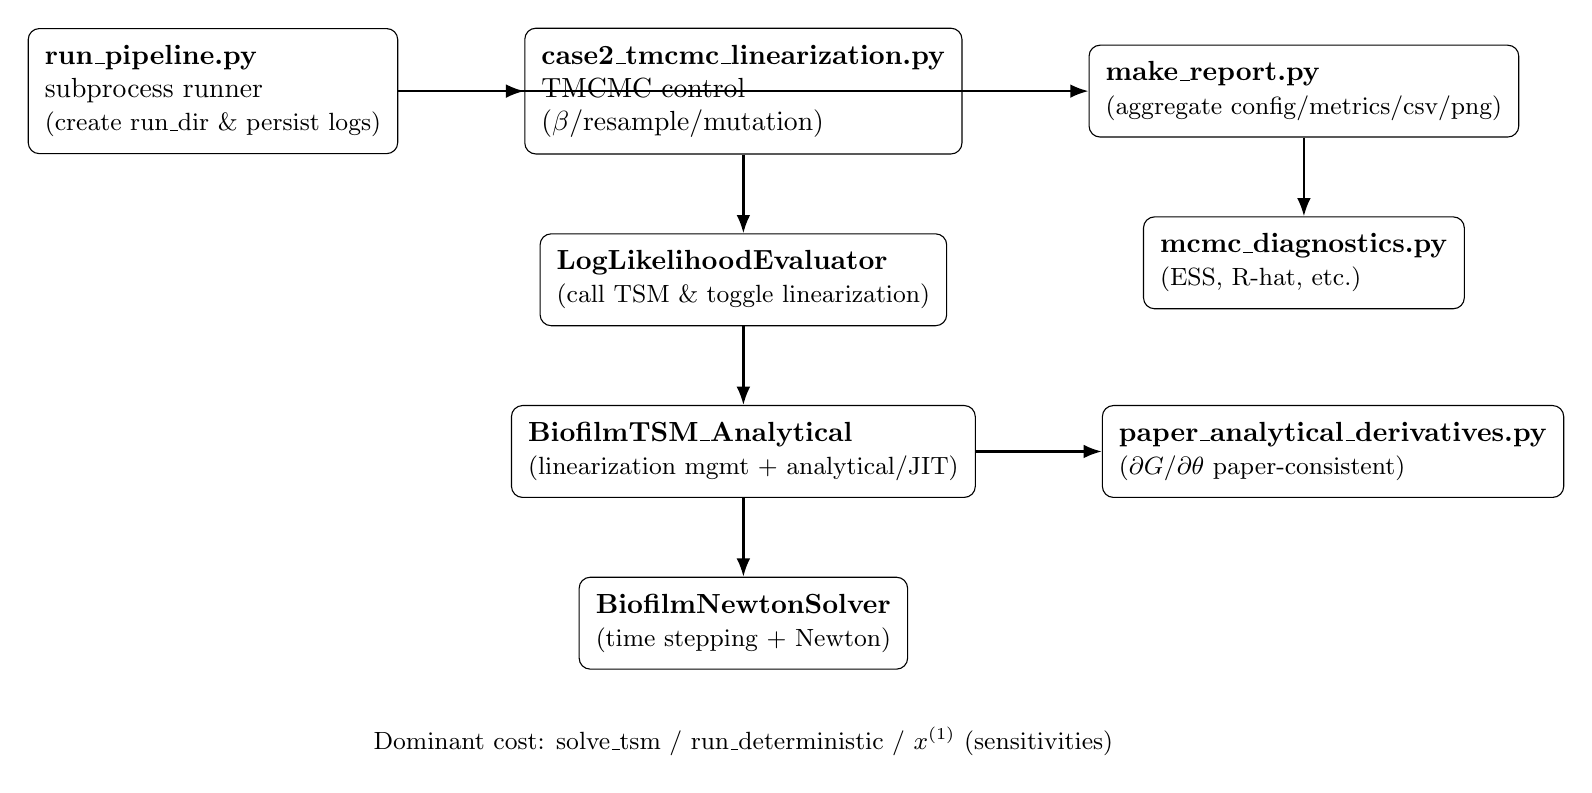
\begin{tikzpicture}[
  node/.style={draw,rounded corners,align=left,inner sep=6pt},
  arrow/.style={-Latex,thick},
  small/.style={font=\small}
]
  \node[node] (pipeline) {\textbf{run\_pipeline.py}\\subprocess runner\\\small(create run\_dir \& persist logs)};
  \node[node,right=16mm of pipeline] (case2) {\textbf{case2\_tmcmc\_linearization.py}\\TMCMC control\\($\beta$/resample/mutation)};
  \node[node,below=10mm of case2] (eval) {\textbf{LogLikelihoodEvaluator}\\\small(call TSM \& toggle linearization)};
  \node[node,below=10mm of eval] (tsm) {\textbf{BiofilmTSM\_Analytical}\\\small(linearization mgmt + analytical/JIT)};
  \node[node,below=10mm of tsm] (solver) {\textbf{BiofilmNewtonSolver}\\\small(time stepping + Newton)};

  \node[node,right=16mm of tsm] (deriv) {\textbf{paper\_analytical\_derivatives.py}\\\small($\partial G/\partial\theta$ paper-consistent)};
  \node[node,right=16mm of case2] (report) {\textbf{make\_report.py}\\\small(aggregate config/metrics/csv/png)};
  \node[node,below=10mm of report] (diag) {\textbf{mcmc\_diagnostics.py}\\\small(ESS, R-hat, etc.)};

  \draw[arrow] (pipeline) -- (case2);
  \draw[arrow] (case2) -- (eval);
  \draw[arrow] (eval) -- (tsm);
  \draw[arrow] (tsm) -- (solver);
  \draw[arrow] (tsm) -- (deriv);
  \draw[arrow] (pipeline) -- (report);
  \draw[arrow] (report) -- (diag);

  \node[small,below=6mm of solver,align=center] (note1)
    {Dominant cost: solve\_tsm / run\_deterministic / $x^{(1)}$ (sensitivities)};
\end{tikzpicture}
\end{center}

\section{End-to-end flow}
\subsection{Pipeline wrapper}
\texttt{run\_pipeline.py} creates a \texttt{run\_dir} and then runs:
\begin{enumerate}[leftmargin=2em]
  \item \texttt{case2\_tmcmc\_linearization.py} (the experiment)
  \item \texttt{make\_report.py} (generate \texttt{REPORT.md} from \texttt{run\_dir})
\end{enumerate}
Combined stdout/stderr are tee'd into \texttt{subprocess.log} under \texttt{run\_dir}.

\subsection{TMCMC loop (high level)}
Conceptual stage loop (implemented in \texttt{run\_TMCMC}):
\begin{enumerate}[leftmargin=2em]
  \item Initialize particles from prior
  \item For stages $s=0,1,\dots$:
  \begin{itemize}
    \item Update $\beta_s \to \beta_{s+1}$ based on target ESS ratio (with min/max $\Delta\beta$)
    \item Evaluate likelihood for each particle (calls TSM)
    \item Update weights $\rightarrow$ normalize $\rightarrow$ compute ESS $\rightarrow$ resample
    \item Mutation (MCMC steps) to restore diversity
    \item Enable linearization (later stages) and update linearization point $\theta_0$ at intervals
  \end{itemize}
  \item Critical: \textbf{ensure $\beta$ reaches 1.0} (look for ``$\beta$ reached 1.0'' in logs)
\end{enumerate}

\subsection{TSM (linearization management + analytical/JIT)}
\texttt{BiofilmTSM\_Analytical.solve\_tsm()} supports:
\begin{itemize}[leftmargin=2em]
  \item \textbf{Linearization OFF} (early exploration): full non-linear TSM evaluation
  \item \textbf{Linearization ON} (later stages): speed up via
        $x(\theta)\approx x(\theta_0)+\frac{\partial x}{\partial\theta}\big|_{\theta_0}(\theta-\theta_0)$
  \item Linearization point update: \texttt{update\_linearization\_point($\theta_{\text{new}}$)} invalidates caches and recomputes
        $x^{(0)}(\theta_0)$ and $x^{(1)}$
\end{itemize}

\subsection{Physical solver (Newton + time stepping)}
\texttt{BiofilmNewtonSolver.run\_deterministic()} integrates the deterministic trajectory;
each step solves a Newton system based on residual $Q$ and Jacobian $J$.
Time-dependent antibiotics are supported via \texttt{alpha\_schedule} (e.g., \texttt{M3\_val}).

\section{Mathematical validation (Hamilton principle $\to$ strong form $\to$ implemented residual)}
We added an explicit math-level validation for the physical model implementation in
\texttt{tmcmc/improved1207\_paper\_jit.py}.
The goal is \textbf{not} to prove the full continuum theory, but to show the following:
\textbf{the paper's strong form equations (biofilm\_simulation, eqs.\ (16)--(18)) reduced to a material point
and discretized by implicit Euler are exactly the same as the residual $Q$ solved by the code}.

\subsection{Paper definitions (model skeleton)}
Let $\phi_i$ be volume fractions, $\psi_i$ be fractions of living cells, and $\bar{\phi}_i=\phi_i\psi_i$ be living biomass.
The holonomic volume constraint is
\[
  f(\phi)=\sum_{l=0}^{n}\phi_l-1=0,
\]
enforced via a Lagrange multiplier $\gamma$.
The free energy density and dissipation potential (paper eqs.\ (10),(14)) are:
\begin{align}
  \Psi(\phi,\psi) &= -\frac12 c^{*} \bar{\phi}^{\mathsf T} A\,\bar{\phi} + \frac12 \alpha^{*} \psi^{\mathsf T} B\,\psi,\\
  \Delta_s(\dot{\bar\phi},\dot\phi) &= \frac12 \dot{\bar\phi}^{\mathsf T}\eta\,\dot{\bar\phi} + \frac12 \dot\phi^{\mathsf T}\eta\,\dot\phi.
\end{align}

\subsection{Strong form (16)--(18) and mapping to residual $Q$}
From the Hamilton principle evaluation, the paper gives (for each species $i$):
\begin{align}
0 &= -c^{*}\psi_i(A\bar{\phi})_i + \eta_i(\dot\phi_i\psi_i^2+\bar{\phi}_i\dot\psi_i+\dot\phi_i) + \gamma, \\
0 &= -c^{*}\phi_i(A\bar{\phi})_i + \alpha^{*} b_i\psi_i + \eta_i(\dot\psi_i\phi_i^2+\bar{\phi}_i\dot\phi_i), \\
0 &= \sum_{l=0}^{n}\phi_l-1.
\end{align}
The implementation uses a material-point model and implicit Euler time discretization
($\dot x \approx (x^{n+1}-x^n)/\Delta t$), and solves \textbf{$Q(g^{n+1})=0$} at each step via Newton.
Key one-to-one correspondences are:
\begin{itemize}[leftmargin=2em]
  \item Interaction term $(A\bar{\phi})_i$: \texttt{Interaction = A @ (phi * psi)}
  \item Constraint: \texttt{Q[9] = sum(phi) + phi0 - 1}
  \item \textbf{$\gamma$ must not appear in the $\psi$ equations} because the constraint depends only on $\phi$ (a mathematical requirement)
\end{itemize}
Additionally, the code includes a \textbf{barrier/penalty term} (coefficient $K_p$) to enforce $0<\phi,\phi_0,\psi<1$
as discussed in the paper.

\subsection{Automated regression checks}
To keep this math-level agreement from regressing, we added pytest checks:
\begin{itemize}[leftmargin=2em]
  \item With barrier disabled ($K_p=0$), the discretized strong form matches the implemented residual $Q$
  \item The $\psi$ equations are independent of $\gamma$
\end{itemize}
Tests live in \texttt{tmcmc/test\_hamilton\_model\_consistency.py};
the detailed note is \texttt{tmcmc/HAMILTON\_VALIDATION.md}.

\section{Accuracy drivers}
The \textbf{likelihood definition} is the top driver (e.g., $\sigma_{\mathrm{obs}}$, variance model).
In particular, including/excluding \textbf{Cov$(\bar\phi,\bar\psi)$ in Var$(\bar\phi\bar\psi)$} can change inference materially.
Keep it audit-able in \texttt{likelihood\_meta\_*.json}.

\paragraph{Why Cov matters (short intuition).}
Even if the observable is the product $\bar\phi\bar\psi$, the uncertainty model depends on whether
fluctuations in $\bar\phi$ and $\bar\psi$ are treated as correlated. Ignoring correlation can lead to
systematic under/over-confidence in the likelihood and thus a materially different posterior.

\paragraph{Note on paper condition mismatch}
Runs with \texttt{--sigma-obs 0.02} will generally not match paper figures that often use 0.01 (not a bug; it changes quantitative fit).

\section{Reproducibility (audit artifacts)}
Minimum artifacts to keep under \texttt{run\_dir}:
\begin{itemize}[leftmargin=2em]
  \item \texttt{config.json}: run configuration, seeds, TMCMC/model params
  \item \texttt{likelihood\_meta\_*.json}: explicit likelihood definition
  \item \texttt{diagnostics\_tables/*.csv}: $\beta$ schedule, acceptance, ROM error, $\theta_0$ history
  \item \texttt{subprocess.log / pipeline.log}: progress + ``$\beta$ reached 1.0''
\end{itemize}

\section{Performance drivers}
Rule of thumb:
\begin{equation}
\text{total time} \approx (\#\text{likelihood evaluations}) \times (\text{cost per TSM evaluation})
\end{equation}
Dominant components:
\begin{itemize}[leftmargin=2em]
  \item \textbf{Largest}: \texttt{BiofilmTSM\_Analytical.solve\_tsm()}
  \item \textbf{Largest}: \texttt{BiofilmNewtonSolver.run\_deterministic()} + \texttt{compute\_Q\_vector()} + \texttt{compute\_Jacobian\_matrix()}
  \item \textbf{Large}: sensitivity generation $x^{(1)}$ (especially when linearization is off)
  \item \textbf{Medium}: TMCMC mechanics (mutation/resample/$\beta$ update)
  \item \textbf{Small}: plotting and I/O (can grow depending on settings)
\end{itemize}

\section{Critical checks}
\begin{itemize}[leftmargin=2em]
  \item \textbf{$\beta=1$ reached}: otherwise you did not reach the posterior
  \item \textbf{NaN/Inf}: ensure no NaN/Inf in solve\_tsm / Newton
  \item \textbf{Complex-step readiness}: \texttt{theta\_to\_matrices} preserves complex dtype
  \item \textbf{Analytical derivative validation}: verify against complex-step reference
\end{itemize}

\section{Common failure modes (symptom $\rightarrow$ likely cause $\rightarrow$ fix)}
\begin{itemize}[leftmargin=2em]
  \item \textbf{$\beta$ never reaches 1.0} $\rightarrow$ too strict ESS target / too few stages $\rightarrow$
        increase \texttt{--n-stages} or relax \texttt{--target-ess-ratio}, check min/max $\Delta\beta$.
  \item \textbf{Low acceptance / frozen mutation} $\rightarrow$ proposal too narrow or linearization too aggressive $\rightarrow$
        increase mutation scale / steps, delay linearization threshold, cap $\|\Delta\theta_0\|$.
  \item \textbf{ROM error spikes after update} $\rightarrow$ $\theta_0$ jump too large $\rightarrow$
        reduce update interval or step cap, add ROM-gated enabling.
  \item \textbf{Posterior too narrow/wide} $\rightarrow$ likelihood variance model mismatch $\rightarrow$
        audit \texttt{likelihood\_meta\_*.json} (especially Cov handling) and $\sigma_{\mathrm{obs}}$.
\end{itemize}

\section{Example figures (auto-picked best run)}
\noindent\textbf{Best run id:} \texttt{\BestRunId}. The following figures are included \emph{if present} under
\texttt{tmcmc/\_runs/\BestRunId}.

\begin{figure}[ht]
  \centering
  \IfFileExists{\BestRunFig{posterior_M1.png}}{
    \includegraphics[width=0.85\linewidth]{\BestRunFig{posterior_M1.png}}
  }{
    \fbox{\parbox{0.85\linewidth}{Missing: \texttt{\BestRunFig{posterior\_M1.png}}}}
  }
  \caption{Posterior for M1 (example).}
\end{figure}

\begin{figure}[ht]
  \centering
  \IfFileExists{\BestRunFig{TSM_simulation_M1_MAP_fit_with_data.png}}{
    \includegraphics[width=0.95\linewidth]{\BestRunFig{TSM_simulation_M1_MAP_fit_with_data.png}}
  }{
    \fbox{\parbox{0.95\linewidth}{Missing: \texttt{\BestRunFig{TSM\_simulation\_M1\_MAP\_fit\_with\_data.png}}}}
  }
  \caption{MAP fit vs data for M1 (example).}
\end{figure}

\begin{figure}[ht]
  \centering
  \IfFileExists{\BestRunAsset{M1_rom_error.png}}{
    \includegraphics[width=0.85\linewidth]{\BestRunAsset{M1_rom_error.png}}
  }{
    % optional
  }
  \IfFileExists{\BestRunAsset{M1_theta0_step_norm.png}}{
    \includegraphics[width=0.85\linewidth]{\BestRunAsset{M1_theta0_step_norm.png}}
  }{
    % optional
  }
  \caption{ROM error and $\|\Delta\theta_0\|$ history (optional diagnostics).}
\end{figure}

\section{Figure ideas (ready-to-use)}
\begin{enumerate}[leftmargin=2em]
  \item TMCMC $\beta$ schedule (per chain)
  \item ROM error at linearization update events (pre/post)
  \item $\|\Delta\theta_0\|$ history (stability of updates)
  \item Cost--accuracy tradeoff (FOM evals or wall-time vs MAP error)
  \item Posterior plots (M1/M2/M3/M3\_val) aligned to paper figures
\end{enumerate}

\section{Appendix: one-sentence summary}
TMCMC stabilizes the transition from prior to posterior while periodically updating the TSM-ROM linearization point,
reducing expensive FOM evaluations without sacrificing estimation accuracy near the MAP.

\section{Related Work}
This work integrates TMCMC (Transitional Markov Chain Monte Carlo) with TSM-ROM (Time-Separated Stochastic Mechanics reduced-order model) to enable efficient Bayesian inference under hybrid uncertainty.
We organize related research by category below.

\subsection{TMCMC (Transitional Markov Chain Monte Carlo)}
TMCMC was proposed by Ching \& Chen (2007) as an MCMC method that achieves gradual transition from prior to posterior via $\beta$ tempering\cite{ChingChen2007TMCMC}.
Compared to conventional MCMC methods, TMCMC is tune-free and naturally provides estimates of model evidence.
Betz et al. (2016) proposed observations and improvements to TMCMC, demonstrating practical performance gains\cite{BetzPapaioannouStraub2016TMCMC}.

Recent extensions include:
\begin{itemize}[leftmargin=2em]
  \item \textbf{X-TMCMC} (Angelikopoulos et al., 2015): Integrates Kriging surrogate models to reduce computational cost\cite{AngelikopoulosPapadimitriouKoumoutsakos2015XTMCMC}.
  \item \textbf{Generalized TMCMC} (Lu et al., 2021): Addresses inefficiencies in tempering schedules for broad applicability\cite{LuKhalilCatanach2021GeneralizedTMCMC}.
  \item \textbf{BASIS} (Wu et al., 2017): An unbiased version of TMCMC that fixes bias issues\cite{WuAngelikopoulosPapadimitriouKoumoutsakos2017BASIS}.
  \item \textbf{CTMCMC} (Ma et al., 2025): Uses copula functions in proposal distributions for complex, high-dimensional distributions\cite{MaPengfeiZhangYi2025CTMCMC}.
\end{itemize}

\subsection{TSM-ROM (Time-Separated Stochastic Mechanics)}
TSM was proposed by Geisler \& Junker (2023) as an efficient uncertainty propagation method that separates time-dependence from stochasticity\cite{GeislerJunker2023TSM}.
Compared to Monte Carlo methods, TSM can estimate expectation and variance with few deterministic simulations.
Geisler et al. (2025) presented a comprehensive TSM framework and demonstrated applicability to inelastic material models\cite{GeislerErdoganNagelJunker2025TSM}.

Key features of TSM:
\begin{itemize}[leftmargin=2em]
  \item Applicable to complex material models with internal variable evolution via separation of time-dependence and stochasticity
  \item Significant computational cost reduction via linear or low-order Taylor expansion
  \item Efficiency achieved through approximation in stochastic parameter space rather than spatial DOF reduction
\end{itemize}

\subsection{Hybrid Uncertainty Quantification}
Bayesian inference under hybrid uncertainty (epistemic + aleatory) faces computational challenges with conventional double-loop procedures.
Beck \& Katafygiotis (1998) established the statistical framework for Bayesian model updating\cite{BeckKatafygiotis1998BMU}.
Kennedy \& O'Hagan (2001) proposed a hybrid uncertainty framework that represents model inadequacy as a statistical discrepancy term\cite{KennedyOHagan2001Calibration}.

Fritsch et al. (2025) achieved Bayesian updating of bacterial biofilms under hybrid uncertainty using TSM-ROM as a surrogate model\cite{Fritsch2025BayesianMicrofilms}.
This work extends that research by integrating TMCMC with TSM-ROM and achieving both accuracy and efficiency through dynamic linearization point updates.

\subsection{Reduced-Order Models for Uncertainty Quantification}
ROM methods for uncertainty quantification are an important research area for computational cost reduction.
Benner et al. (2015) provided a survey of projection-based ROM methods for parametric dynamical systems\cite{BennerGugercinWillcox2015ROM}.
Peherstorfer et al. (2018) provided a survey of multifidelity methods for UQ\cite{PeherstorferWillcoxGunzburger2018ROMUQ}.

Polynomial Chaos Expansion (Xiu \& Karniadakis, 2002) is a method that efficiently performs UQ via expansion in stochastic parameter space\cite{XiuKarniadakis2002PolynomialChaos}.
TSM is similar to this approach but is particularly applicable to inelastic material models through separation of time-dependence and stochasticity.

\subsection{Bayesian Inference and MCMC Methods}
The foundation of MCMC methods dates back to the Metropolis algorithm (Metropolis et al., 1953) and the Metropolis-Hastings algorithm (Hastings, 1970)\cite{MetropolisRosenbluthRosenbluthTellerTeller1953,Hastings1970MCMC}.
Sequential Monte Carlo (Del Moral et al., 2006) provides a similar approach to TMCMC via population-based sampling\cite{DelMoralDoucetJasra2006SMC}.

\subsection{Surrogate Models and Emulators}
As alternatives to expensive physical models, surrogate models such as Gaussian Process Regression (Rasmussen \& Williams, 2006) and Bayesian Emulation (Conti \& O'Hagan, 2010) are used\cite{RasmussenWilliams2006GPR,ContiOHagan2009BayesianEmulation}.
This work uses TSM-ROM as a surrogate model, achieving both accuracy and efficiency through analytical sensitivity computation compared to GP-based methods.

\subsection{Adaptive Surrogate Models and Active Learning}
Recent work has focused on adaptive surrogate models with active learning.
Villani et al. (2024) proposed adaptive GP surrogates using KL divergence-based acquisition criteria, reducing forward model evaluations\cite{Villani2024AdaptiveGP}.
Xu et al. (2024) proposed GP surrogates for multimodal posteriors combined with ensemble smoothers\cite{Xu2024AdaptiveGPMultimodal}.
Meles et al. (2025) achieved two orders of magnitude computational savings through sequential surrogate refinement with posterior-guided training\cite{Meles2025SequentialSurrogateRefinement}.
Scheurer et al. (2025) proposed UA-SABI (Uncertainty-Aware Surrogate-based Amortized Bayesian Inference) with explicit surrogate uncertainty modeling\cite{Scheurer2025UASABI}.

\subsection{Adaptive Tempering Schedules and ESS-based Methods}
Research on ESS-based adaptive tempering schedules has advanced.
Zhao \& Pillai (2024) optimized temperature ladders using policy gradients with ACT/ESS as metrics\cite{ZhaoPillai2024PolicyGradientPT}.
Peña \& Jenkins (2025) proposed reddemcee, achieving adaptive tempering based on multiple objectives including ESS-based metrics\cite{PenaJenkins2025Reddemcee}.
Li et al. (2024) analyzed the optimality of swap acceptance rate $\approx$ 0.234 across dimensions and tuning regimes\cite{LiWangDouRosenthal2024TemperatureSpacing}.
Wang et al. (2025) combined normalizing flows with ESS-based adaptive annealing schedules, achieving approximately 10$\times$ computational savings\cite{WangChiDinner2025NormalizingFlowsESS}.

\subsection{Adaptive Linearization Point Updates in ROMs}
Research on adaptive linearization point updates in ROMs has also advanced.
Farhat et al. (2020) achieved in-situ adaptive reduction with libraries of local ROBs and online updates\cite{AdaptiveROM2020InSitu}.
MORe DWR (2024) proposed incremental POD with dual-weighted residual (DWR) error estimators, updating linearization points incrementally\cite{AdaptiveROM2024DWR}.
Goal-oriented adaptive sampling (2025) proposed sampling new linearization points based on error to maintain ROM validity\cite{AdaptiveROM2025GoalOriented}.
Interpolated adaptive linear ROM (2025) proposed dynamically adjusting linearization mappings via Grassmann interpolation\cite{AdaptiveROM2025Interpolated}.

\subsection{Biofilm Modeling with Bayesian Inference}
Applications of Bayesian inference to biofilm modeling have also progressed.
A 2023 study performed Bayesian estimation of viscoelastic parameters for \textit{Pseudomonas aeruginosa} biofilms using MCMC to estimate posterior distributions\cite{Biofilm2023Viscoelastic}.
These studies demonstrate the applicability of our biofilm model approach.

\subsection{Positioning of This Work}
This work extends and integrates existing research in the following ways:
\begin{itemize}[leftmargin=2em]
  \item \textbf{Integration of TMCMC and TSM-ROM}: Combines both methods to enable efficient Bayesian inference under hybrid uncertainty
  \item \textbf{Dynamic linearization point updates}: Maintains first-order approximation accuracy of TSM-ROM by updating linearization points near MAP in later TMCMC stages (related to adaptive ROM research)
  \item \textbf{ESS-targeted $\Delta\beta$ control}: Adaptive tempering schedule based on ESS targets rather than fixed schedules (related to adaptive tempering research)
  \item \textbf{Practical improvements}: Implements practical enhancements such as K-step mutation and observation-based linearization point selection
  \item \textbf{Surrogate uncertainty consideration}: Monitors TSM-ROM error and controls timing of linearization point updates (related to UA-SABI research)
\end{itemize}

\section{References}
\begin{thebibliography}{99}
\bibitem{Fritsch2025BayesianMicrofilms}
Fritsch, L., Geisler, H., Grashorn, J., Klempt, F., Soleimani, M., Broggi, M., Junker, P., Beer, M.
\textit{Bayesian updating of bacterial microfilms under hybrid uncertainties with a novel surrogate model}.
(Local PDF: \localpath{tmcmc/Bayesian updating of bacterial microfilms under hybrid uncertainties with a novel surrogate model - Kopie.pdf}).

\bibitem{Klempt2025ContinuumBiofilm}
Klempt, F., Geisler, H., Soleimani, M., Junker, P.
\textit{A continuum multi-species biofilm model with a novel interaction scheme}. arXiv:2509.01274v1, 2025-09-01.
(Local PDF: \localpath{tmcmc/biofilm\_simulation.pdf}).

\bibitem{JunkerBalzani2021ExtendedHamilton}
Junker, P., Balzani, D.
\textit{An extended Hamilton principle as unifying theory for coupled problems and dissipative microstructure evolution}.
Continuum Mechanics and Thermodynamics, 33(4), 1931--1956 (2021). DOI: \doi{10.1007/s00161-021-01017-z}.
(Local PDF: \localpath{tmcmc/hamiltonian.pdf}).

\bibitem{Heine2025PeriImplant}
Heine, N., Bittroff, K., Szafrański, S. P., Duitscher, M., Behrens, W., Vollmer, C., Mikolai, C., Kommerein, N., Debener, N., Frings, K., Heisterkamp, A., Scheper, T., Torres-Mapa, M. L., Bahnemann, J., Stiesch, M., Doll-Nikutta, K.
\textit{Influence of species composition and cultivation condition on peri-implant biofilm dysbiosis in vitro}.
Frontiers in Oral Health, 6:1649419 (2025). DOI: \doi{10.3389/froh.2025.1649419}.
(Local PDF: \localpath{tmcmc/Influence of species composition and cultivation condition on peri-implant biofilm dysbiosis in vitro.pdf}).

\bibitem{ChingChen2007TMCMC}
Ching, J., Chen, Y.-C.
\textit{Transitional Markov Chain Monte Carlo Method for Bayesian Model Updating, Model Class Selection, and Model Averaging}.
Journal of Engineering Mechanics, 133(7), 816--832 (2007). DOI: \doi{10.1061/(ASCE)0733-9399(2007)133:7(816)}.

\bibitem{BetzPapaioannouStraub2016TMCMC}
Betz, W., Papaioannou, I., Straub, D.
\textit{Transitional Markov Chain Monte Carlo: Observations and Improvements}.
Journal of Engineering Mechanics, 142(5), 04016016 (2016). DOI: \doi{10.1061/(ASCE)EM.1943-7889.0001066}.

\bibitem{GeislerJunker2023TSM}
Geisler, H., Junker, P.
\textit{Time-separated stochastic mechanics for the simulation of viscoelastic structures with local random material fluctuations}.
Computer Methods in Applied Mechanics and Engineering, 407, 115916 (2023). DOI: \doi{10.1016/j.cma.2023.115916}.

\bibitem{GeislerErdoganNagelJunker2025TSM}
Geisler, H., Erdogan, C., Nagel, J., Junker, P.
\textit{A new paradigm for the efficient inclusion of stochasticity in engineering simulations: Time-separated stochastic mechanics}.
Computational Mechanics, 75(1), 211--235 (2025). DOI: \doi{10.1007/s00466-024-02500-5}.

\bibitem{AngelikopoulosPapadimitriouKoumoutsakos2015XTMCMC}
Angelikopoulos, P., Papadimitriou, C., Koumoutsakos, P.
\textit{X-TMCMC: Adaptive Kriging for Bayesian Inverse Problems}.
Computer Methods in Applied Mechanics and Engineering, 289, 409--428 (2015). DOI: \doi{10.1016/j.cma.2015.02.011}.

\bibitem{LuKhalilCatanach2021GeneralizedTMCMC}
Lu, D., Khalil, M., Catanach, T. et al.
\textit{Generalized Transitional Markov Chain Monte Carlo for Bayesian Inverse Problems}.
arXiv preprint arXiv:2112.02180 (2021).

\bibitem{WuAngelikopoulosPapadimitriouKoumoutsakos2017BASIS}
Wu, S., Angelikopoulos, P., Papadimitriou, C., Koumoutsakos, P.
\textit{BASIS: Bayesian Annealed Sequential Importance Sampling}.
Journal of Computational Physics, 335, 289--299 (2017). DOI: \doi{10.1016/j.jcp.2017.01.010}.

\bibitem{MaPengfeiZhangYi2025CTMCMC}
Ma, P., Zhang, Y., Cai, E., Luo, M., Guo, X.
\textit{Copula-based Transitional Markov Chain Monte Carlo for Bayesian Model Updating}.
Reliability Engineering \& System Safety, 265, 110772 (2025). DOI: \doi{10.1016/j.ress.2025.110772}.

\bibitem{Villani2024AdaptiveGP}
Villani, M. et al.
\textit{Adaptive Gaussian Process Regression for Bayesian Inverse Problems}.
arXiv preprint arXiv:2404.19459 (2024).

\bibitem{Xu2024AdaptiveGPMultimodal}
Xu, W. et al.
\textit{Adaptive Gaussian Process for Multi-modal Bayesian Inverse Problems}.
arXiv preprint arXiv:2409.15307 (2024).

\bibitem{Meles2025SequentialSurrogateRefinement}
Meles, G. A. et al.
\textit{Bayesian Full Waveform Inversion with Sequential Surrogate Model Refinement}.
arXiv preprint arXiv:2505.03246 (2025).

\bibitem{Scheurer2025UASABI}
Scheurer, M. et al.
\textit{Uncertainty-Aware Surrogate-based Amortized Bayesian Inference (UA-SABI)}.
arXiv preprint arXiv:2505.08683 (2025).

\bibitem{ZhaoPillai2024PolicyGradientPT}
Zhao, T., Pillai, N. S.
\textit{Policy Gradients for Optimal Parallel Tempering MCMC}.
arXiv preprint arXiv:2409.01574 (2024).

\bibitem{PenaJenkins2025Reddemcee}
Peña, J., Jenkins, D.
\textit{reddemcee: Adaptive Parallel Tempering Ensemble Sampler}.
arXiv preprint arXiv:2509.24870 (2025).

\bibitem{LiWangDouRosenthal2024TemperatureSpacing}
Li, Y., Wang, Y., Dou, Z., Rosenthal, J. S.
\textit{Temperature Spacing via Swap Acceptance $\approx$ 0.234}.
arXiv preprint arXiv:2408.06894 (2024).

\bibitem{WangChiDinner2025NormalizingFlowsESS}
Wang, Y., Chi, C., Dinner, A. R.
\textit{Normalizing Flows + Annealing with ESS-based Adaptive Schedule}.
arXiv preprint arXiv:2505.03652 (2025).

\bibitem{AdaptiveROM2020InSitu}
Farhat, C. et al.
\textit{In-situ Adaptive Reduction of Nonlinear Multiscale Structural Dynamics}.
arXiv preprint arXiv:2004.00153 (2020).

\bibitem{AdaptiveROM2024DWR}
\textit{Adaptive Space-Time Model Order Reduction with Dual-Weighted Residual (MORe DWR)}.
Archive of Applied Mechanics (2024). DOI: \doi{10.1186/s40323-024-00262-6}.

\bibitem{AdaptiveROM2025GoalOriented}
\textit{Goal-oriented Adaptive Sampling for Projection-based ROMs}.
Computers \& Structures (2025).

\bibitem{AdaptiveROM2025Interpolated}
\textit{Interpolated Adaptive Linear ROM for Deformation Dynamics}.
arXiv preprint arXiv:2509.25392 (2025).

\bibitem{Biofilm2023Viscoelastic}
\textit{Viscoelastic Properties of Pseudomonas aeruginosa Biofilms: Bayesian Estimation}.
Biophysical Reports, 3, 100130 (2023). DOI: \doi{10.1016/j.bpr.2023.100130}.

\bibitem{BeckKatafygiotis1998BMU}
Beck, J. L., Katafygiotis, L. S.
\textit{Updating Models and Their Uncertainties. I: Bayesian Statistical Framework}.
Journal of Engineering Mechanics, 124(4), 455--461 (1998). DOI: \doi{10.1061/(ASCE)0733-9399(1998)124:4(455)}.

\bibitem{KennedyOHagan2001Calibration}
Kennedy, M. C., O'Hagan, A.
\textit{Bayesian Calibration of Computer Models}.
Journal of the Royal Statistical Society: Series B, 63(3), 425--464 (2001). DOI: \doi{10.1111/1467-9868.00294}.

\bibitem{BennerGugercinWillcox2015ROM}
Benner, P., Gugercin, S., Willcox, K.
\textit{A Survey of Projection-Based Model Reduction Methods for Parametric Dynamical Systems}.
SIAM Review, 57(4), 483--531 (2015). DOI: \doi{10.1137/130932715}.

\bibitem{PeherstorferWillcoxGunzburger2018ROMUQ}
Peherstorfer, B., Willcox, K., Gunzburger, M.
\textit{Survey of Multifidelity Methods for Uncertainty Quantification, Propagation, and Optimization}.
SIAM Review, 60(3), 550--591 (2018). DOI: \doi{10.1137/16M1082469}.

\bibitem{XiuKarniadakis2002PolynomialChaos}
Xiu, D., Karniadakis, G. E.
\textit{The Wiener--Askey Polynomial Chaos for Stochastic Differential Equations}.
SIAM Journal on Scientific Computing, 24(2), 619--644 (2002). DOI: \doi{10.1137/S1064827501387826}.

\bibitem{MetropolisRosenbluthRosenbluthTellerTeller1953}
Metropolis, N., Rosenbluth, A. W., Rosenbluth, M. N., Teller, A. H., Teller, E.
\textit{Equation of State Calculations by Fast Computing Machines}.
The Journal of Chemical Physics, 21(6), 1087--1092 (1953). DOI: \doi{10.1063/1.1699114}.

\bibitem{Hastings1970MCMC}
Hastings, W. K.
\textit{Monte Carlo Sampling Methods Using Markov Chains and Their Applications}.
Biometrika, 57(1), 97--109 (1970). DOI: \doi{10.1093/biomet/57.1.97}.

\bibitem{DelMoralDoucetJasra2006SMC}
Del Moral, P., Doucet, A., Jasra, A.
\textit{Sequential Monte Carlo Samplers}.
Journal of the Royal Statistical Society: Series B, 68(3), 411--436 (2006). DOI: \doi{10.1111/j.1467-9868.2006.00553.x}.

\bibitem{RasmussenWilliams2006GPR}
Rasmussen, C. E., Williams, C. K. I.
\textit{Gaussian Processes for Machine Learning}.
MIT Press (2006). ISBN: 026218253X.

\bibitem{ContiOHagan2009BayesianEmulation}
Conti, S., O'Hagan, A.
\textit{Bayesian Emulation of Complex Multi-Output and Dynamic Computer Models}.
Journal of Statistical Planning and Inference, 140(3), 640--651 (2010). DOI: \doi{10.1016/j.jspi.2009.08.006}.
\end{thebibliography}

\end{document}
